\chapter{Requisiti Software}
\raggedright{\section{Modellazione casi d'uso richiesti}}
All'interno della nostra applicazione rimodernizzata, da qui in avanti chiamata \gls{Alexandria}, abbiamo individuato 6 \gls{casi d'uso}: un caso d'uso relativo all'autenticazione, un caso d'uso relativo alla ricerca di un \gls{riferimento} e di un \gls{autore}, un caso d'uso relativo alla creazione dei riferimenti, un caso d'uso relativo alla creazione di una \gls{categoria}, un caso d'uso relativo alla visualizzazione e creazione modifica dei propri riferimenti e infine caso d'uso relativo alle impostazioni utente.
\begin{figure}[H]
    \centering
        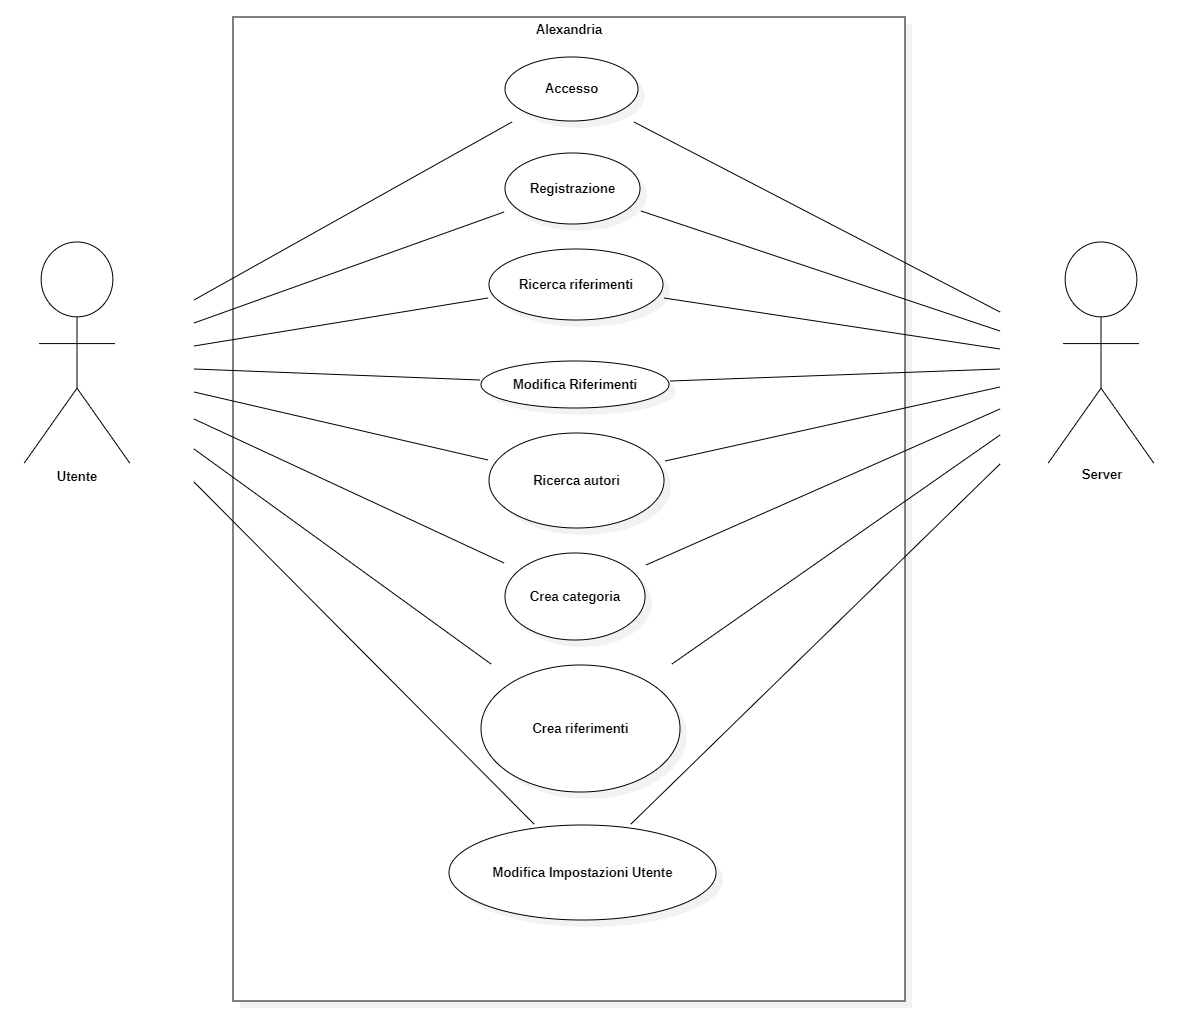
\includegraphics[width=.90\textwidth]{Immagini/Alexandria/useCase.png} 
    \caption{Use Case Diagram di Alexandria}
\end{figure}

\newpage
Spiegazione dettagliata dei casi d'uso mostrati: 
\begin{itemize}
    \item Il caso d'uso \textit{Accesso} permette l'autenticazione di un utente, ovvero permette ad un utente di accedere al sistema inserendo le proprie credenziali (scelte dall'utente stesso durante la fase di registrazione).
    \item  Il caso d'uso \textit{Registrazione} permette di registrare un nuovo utente al sistema, scegliendo un proprio username, una propria password e una email.
    \item Il caso d'uso \textit{Ricerca Riferimenti} permette ad un utente di cercare un riferimento esistente nel sistema. Se inesistente, il sistema notifica l'utente dell'inesistenza del riferimento cercato, altrimenti permette di visualizzarlo. 
    \item Il caso d'uso \textit{Modifica Riferimenti} permette ad un utente di modificare un riferimento creato in precedenza, in particolare permette di modificare un \gls{attributo} inserito in precedenza,  potendo scegliere un nuovo valore. 
    \item  Il caso d'uso \textit{Ricerca autori} permette all'utente di ricercare un autore in particolare e tutte le sue opere pubblicate presenti nel sistema.
    \item Il caso d'uso \textit{Crea categoria} permette all'utente di creare una categoria e di poter scegliere un'eventuale \gls{sopra-categoria}.
    \item  Il caso d'uso \textit{Crea Riferimenti} permette ad un utente di creare un riferimento e di poterne assegnare gli attributi. 
    \item Infine, il caso d'uso \textit{Modifica Impostazioni utente} permette ad un utente di modificare tutte le informazioni inserite durante la fase di registrazione.
\end{itemize}
Tutte queste funzionalità richiedono un attore esterno, ovvero il Server, il quale permette di registrare ogni modifica al sistema. Sostanzialmente, senza di esso l'applicativo non può funzionare correttamente.


\raggedright{\section{Individuazione target degli utenti}}
Il target principale degli utenti sono coloro i quali intendono gestire e visualizzare i propri riferimenti bibliografici. Per tale motivo Alexandria permette la gestione e la visualizzazione affidabile dei riferimenti creati. In aggiunta, è possibile visualizzare i riferimenti degli altri utenti presenti nel sistema.
Un altro possibile target di utenti sono gli autori stessi dei riferimenti bibliografici, poiché possono gestire facilmente le proprie opere pubblicate e visualizzarne gli attributi.
Un altro target di utenti sono le case editrici che intendono gestire le varie edizioni dei propri riferimenti pubblicati. 
Considerando tutti i possibili utenti, il team si impegna di poter soddisfare tutte le esigenze degli usufruitori e di poter garantire un'eccellente usabilità e affidabilità del sistema.

\raggedright{\section{Casi d'uso significativi nel dettaglio}}
\label{casiUso}
Vengono qui riportati quattro casi d'uso significativi nel dettaglio utilizzando il template di Cockburn. La sezione \textit{Descrizione}, presente in tutte le tabelle, indica lo scenario di successo. Le estensioni indicano uno scenario di falllimento o tipi di errore. Lo scenario sottovariante indica una variante del caso di successo.
\raggedright{\subsection{Caso d'uso: Ricerca Riferimenti}}

\begin{table}[H]    

\def\arraystretch{1.5}

\begin{tabularx}{\linewidth}{|l|X|X|X|}

  \hline Caso d'Uso 1 & \multicolumn{3} {l|}{Ricerca di un riferimento} \\ \hline Obiettivo & \multicolumn{3}{>{\hsize=\dimexpr 3\hsize+4\tabcolsep+2\arrayrulewidth\relax}X|}{%
    L'obiettivo principale è quello di ricercare uno o più riferimenti inserendo attributi specifici} \\
 \hline Precondizioni &
  \multicolumn{3}{l|}{L'utente deve essere stato correttamente registrato in precedenza.} \\
 \hline Condizioni di successo &
  \multicolumn{3}{l|}{L'utente trova e visualizza il riferimento desiderato} \\
 \hline Condizioni di fallimento &
  \multicolumn{3}{l|}{L'utente non trova il riferimento desiderato poiché inesistente} \\
 \hline Attore principale &
  \multicolumn{3}{l|}{Utente registrato} \\
 \hline Trigger & \multicolumn{3}{l|}{Utente preme su \textit{Ricerca} nella Homepage.} \\

  \hline \multirow{2}{*}{Descrizione} & Step & Attore & Sistema \\

  \cline{2-4} &  1 & Inserisce titolo del riferimento & \\
  \cline{2-4} &  2 & Seleziona uno dei \gls{tipi di riferimento} disponibili & \\
  \cline{2-4} &  3 &  & Seleziona i tipi di riferimento scelti \\
  \cline{2-4} &  4 & Cerca una categoria apposita &  \\
  \cline{2-4} &  5 &  & Mostra le categorie cercate dall'utente \\
  \cline{2-4} &  6 & Seleziona il \gls{tipo di ricerca} & \\
  \cline{2-4} &  7 & & Deselziona i tipi di ricerca non scelti dall'utente \\
  \cline{2-4} &  8 & Preme su ricerca & \\
  \cline{2-4} &  9 &  & Mostra frame \textit{Risultati ricerca} \\
  \cline{2-4} &  10 & Seleziona ordine ricerca & \\
  \cline{2-4} &  11 &  & Ordina ricerca per il tipo selezionato dall'utente \\
  \cline{2-4} &  12 & Seleziona un riferimento & \\
  \cline{2-4} &  13 &  & Mostra frame \textit{Visualizza Citazione}\\
   \hline Note & \multicolumn{3}{l|}{I nomi dei \textit{frame} provengono dai MockUp realizzati su Figma.} \\
 \hline

    \end{tabularx}
    \end{table}
    
    \newpage
    
\begin{table}[H]
\def\arraystretch{1.5}
\begin{tabularx}{\linewidth}{|p{5.5cm}@{}|X|X|X|}
        
 \hline \multirow{2}{*}{\shortstack[l]{Extension A: \\ L'utente torna indietro}} & Step &
  Attore & Sistema \\
 \cline{2-4} & D.1 a D.7 & Preme su \textit{Indietro} & \\
 \cline{2-4} &  A.1 &  & Mostra frame \textit{HomePage} \\
 \hline
  \multirow{2}{*}{\shortstack[l]{Extension B: \\ L'utente non inserisce il testo}} & Step & Attore & Sistema \\

  \cline{2-4} & D.1 a D.7 & Preme su ricerca & \\
  \cline{2-4} & B.1 &  & Mostra tutti i riferimenti esistenti \\
 \hline
  \multirow{2}{*}{\shortstack[l]{Extension C: \\ Non esistono i \\ riferimenti ricercati}} & Step & Attore & Sistema \\

  \cline{2-4} & D.8 + D.9 & Preme su ricerca & \\
  \cline{2-4} & C.1  &  & Mostra frame \textit{Ricerca Vuota} \\
  \cline{2-4} & C.2  & Preme su Crea &  \\
  \cline{2-4} & C.3  & & Mostra frame \textit{Crea Modifica Citazione}  \\
  \cline{2-4} & C.2  & Seleziona Indietro &  \\
  \cline{2-4} & C.4  & & Ritorna a frame \textit{Ricerca}  \\

 \hline Note & \multicolumn{3}{l|}{I nomi dei \textit{frame} provengono dai MockUp realizzati su Figma.} \\
 \hline


\end{tabularx}
\end{table}
\raggedright{\subsection{Caso d'uso: Creazione Riferimento}}

\begin{table}[H]
\def\arraystretch{1.3}
\begin{tabularx}{\linewidth}{|l|p{5.5cm}@{}|X|X|}

  \hline Caso d'Uso 2 & \multicolumn{3} {l|}{Creazione di un Riferimento} \\ \hline Obiettivo & \multicolumn{3}{>{\hsize=\dimexpr 3\hsize+4\tabcolsep+2\arrayrulewidth\relax}X|}{%
    L'obiettivo principale è quello di creare un nuovo riferimento visualizzabile per tutti gli utenti.} \\
 \hline Precondizioni &
  \multicolumn{3}{l|}{L'utente deve essere stato correttamente registrato in precedenza} \\
 \hline Condizioni di successo &
  \multicolumn{3}{l|}{\shortstack[l]{Viene creato un nuovo riferimento nel sistema, \\ visualizzabile
    per tutti gli utenti.}} \\
 \hline Condizioni di fallimento &
  \multicolumn{3}{l|}{Il riferimento è già esistente nel sistema.} \\
 \hline Attore principale &
  \multicolumn{3}{l|}{Utente registrato} \\
 \hline Trigger & \multicolumn{3}{l|}{Utente preme su \textit{Crea Riferimento} nella barra di controllo} \\

  \hline \multirow{2}{*}{Descrizione} & Step & Attore & Sistema \\

  \cline{2-4} & 1 & Inserisce titolo citazione & \\
  \cline{2-4} & 2 & Preme sull'icona \textit{Data} & \\
  \cline{2-4} & 3 & & Mostra dialog \textit{Crea Modifica Citazione Data}\\
  \cline{2-4} & 4 & Sceglie una data e preme Ok & \\
  \cline{2-4} & 5 & & Ritorna al frame \textit{Crea Modifica Citazione} \\
  \cline{2-4} & 6 & Preme su Riferimento a & \\
  \cline{2-4} & 7 & & Mostra dialog \textit{Crea Modifica Citazione Riferimento a} \\
  \cline{2-4} & 8 & Cerca o sceglie un riiferimento e preme Ok & \\
  \cline{2-4} & 9 & & Ritorna al frame \textit{Crea Modifica Citazione} \\
  \cline{2-4} & 10 & Seleziona il tipo di riferimento & \\
  \cline{2-4} & 11 & & Deseleziona i tipi di riferimento non scelti dall'utente \\
  \cline{2-4} & 12 & Preme su Descrizione & \\
    \hline Note & \multicolumn{3}{l|}{I dialog sono descritti come \textit{Frame} su Figma.} \\
   \hline

  \end{tabularx}
\end{table}



\begin{table}[H]
\def\arraystretch{1.3}
\begin{tabularx}{\linewidth}{|l|p{5.5cm}@{}|X|X|}
\hline
  \cline{2-4} & 13 & & Mostra dialog \textit{Crea Modifica Citazione Descrizione}\\

  \cline{2-4} & 14 & Inserisce una descrizione, un DOI, una edizione e numero delle pagine e preme Ok& \\
  \cline{2-4} & 15 & & Ritorna al frame \textit{Crea Modifica Citazione} \\
  \cline{2-4} & 16 & Preme su Link & \\
  \cline{2-4} & 17 & & Mostra dialog \textit{Crea Modifica Citazione Link} \\
  \cline{2-4} & 18 & Inserisce URL e preme Salva & \\
  \cline{2-4} & 19 & & Ritorna al frame \textit{Crea Modifica Citazione} \\
  \cline{2-4} & 20 & Inserisce i valori per \textit{Editore}, \textit{Luogo}, \textit{ISSN} e \textit{ISBN} e preme su conferma & \\
  \cline{2-4} & 21 & & Mostra frame \textit{Crea Modifica Citazione Successo} \\
  \cline{2-4} & 22 & Preme su Visualizza & \\
  \cline{2-4} & 23 & & Mostra frame \textit{Visualizza Citazione} \\
   \hline Note & \multicolumn{3}{l|}{I dialog sono descritti come \textit{Frame} su Figma.} \\
   \hline

  \end{tabularx}
\end{table}
  
\newpage

\begin{table}[H]
  \def\arraystretch{1.1}
  \begin{tabularx}{\linewidth}{|p{6.4cm}@{}|X|X|X|}
      
 \hline \multirow{2}{*}{\shortstack[l]{Extension A: \\  Riferimento già esistente}} & Step &
  Attore & Sistema \\
 \cline{2-4} &  D.20 & & Mostra dialog \textit{Crea Modifica Citazione Errore} \\
 \cline{2-4} & A.1 & Attende pochi secondi & \\
\cline{2-4} & A.2 & & Ritorna sul frame \textit{Crea Modifica Citazione} \\
 \hline
 
  \multirow{2}{*}{\shortstack[l]{Extension B:\\ Riferimento connesso non esistente}} & Step & Attore & Sistema \\
  \cline{2-4} & D.7 & Inserisce un riferimento non esistente e preme Ok & \\
  \cline{2-4} & B.1 & & Mostra snackbar \textit{Errore Modifica Citazione Riferimento a} \\

 \hline
 
  \multirow{2}{*}{Extension C: Riferimento nullo} & Step & Attore & Sistema \\
  \cline{2-4} & D.7 & Lascia un campo vuoto e preme Ok & \\
  \cline{2-4} & C.1 & & Mostra snackbar \textit{Errore Modifica Citazione Riferimento a} \\

 \hline Note & \multicolumn{3}{l|}{} \\
 \hline


\end{tabularx}
\end{table}
\begin{table}[H]
  \def\arraystretch{1.1}
  \begin{tabularx}{\linewidth}{|p{6.4cm}@{}|X|X|X|}
  \hline
  \multirow{2}{*}{Extension E: URL non valido} & Step & Attore & Sistema \\
  \cline{2-4} & D.17 & Inserisce un link non valido e preme Ok & \\
  \cline{2-4} & E.1 & & Mostra snackbar \textit{Errore Crea Modifica Citazione Link} \\

 \hline
 
  \multirow{2}{*}{\shortstack[l]{Extension F: \\ Descrizione non valida}} & Step & Attore & Sistema \\
  \cline{2-4} & D.13 & Inserisce valori non validi per la descrizione, pagine, edizione o DOI e preme Ok & \\
  \cline{2-4} & F.1 & & Mostra snackbar \textit{Errore Crea Modifica Citazione Descrizione} \\
  \cline{2-4} & F.2 & & Scomparsa della snackbar \\

 \hline
 
  \multirow{2}{*}{Extension G: Campi tutti vuoti} & Step & Attore & Sistema \\
  \cline{2-4} & G.1 & Non inserisce nessun valore e preme su Conferma & \\
  \cline{2-4} & G.2 & & Mostra dialog \textit{Crea Modifica Citazione Errore} \\
  \cline{2-4} & G.3 & & Ritorna sul frame \textit{Crea Modifica Citazione} \\

 \hline Note & \multicolumn{3}{l|}{} \\
 \hline


\end{tabularx}
\end{table}

\newpage
\raggedright{\subsection{Caso d'uso: Modifica propri Riferimenti}}
\begin{table}[H]
\def\arraystretch{1.5}
\begin{tabularx}{\linewidth}{|l|X|X|X|}

  \hline Caso d'Uso 3 & \multicolumn{3} {l|}{Modifica dei propri riferimenti creati} \\ \hline Obiettivo & \multicolumn{3}{>{\hsize=\dimexpr 3\hsize+4\tabcolsep+2\arrayrulewidth\relax}X|}{%
    Poter modificare un proprio riferimento creato e poter visualizzare le modifiche correttamente. } \\
 \hline Precondizioni &
  \multicolumn{3}{l|}{Utente deve essere correttamente registrato} \\
 \hline Condizioni di successo &
  \multicolumn{3}{l|}{Modificare correttamente il riferimento} \\
 \hline Condizioni di fallimento &
  \multicolumn{3}{l|}{I nuovi valori inseriti non sono validi} \\
 \hline Attore principale &
  \multicolumn{3}{l|}{Utente registrato} \\
 \hline Trigger & \multicolumn{3}{l|}{L'utente preme su \textit{Mie Citazioni}} \\

  \hline \multirow{2}{*}{Descrizione} & Step & Attore & Sistema \\

  \cline{2-4} & 1 & Cerca titolo di una citazione & \\
  \cline{2-4} & 2 &  & Mostra l'eventuale riferimento specificato \\
  \cline{2-4} & 3 & Preme su Ordina per & \\
  \cline{2-4} & 4 &  & Ordina i riferimenti per l'ordine specificato \\
  \cline{2-4} & 5 & Seleziona un riferimento & \\
  \cline{2-4} & 6 &  & Evidenzia il riferimento selezionato\\
  \cline{2-4} & 7 & Preme su Modifica & \\
  \cline{2-4} & 8 &  & Mostra dialog \textit{Visualizza Propri Riferimenti Conferma Modifica} \\
  \cline{2-4} & 9 & Preme su Modifica & \\
  \cline{2-4} & 10 &  & Mostra frame \textit{Crea Modifica Riferimento} \\
  \cline{2-4} & 11 & Modifica il proprio riferimento e preme su Conferma & \\
  \cline{2-4} & 12 &  & Mostra dialog \textit{Crea Modifica Citazione Successo}\\
  \cline{2-4} & 13 & Preme su visualizza & \\
  \cline{2-4} & 14 &  & Mostra frame \textit{Visualizza Citazione} \\

\hline
\end{tabularx}
\end{table}


\begin{table}[H]
\def\arraystretch{1.5}
\begin{tabularx}{\linewidth}{|l|X|X|X|}
 
 \hline \multirow{2}{6cm}{Extension A: L'utente seleziona non seleziona un riferimento} & Step &
  Attore & Sistema \\
 \cline{2-4} & D.7 & & Mostra dialog \textit{Errore Visualizza Propri Riferimenti Selezione} \\
 \cline{2-4} & A.1 & & Ritorna su \textit{Visualizza Propri Riferimenti} \\
 \hline
  \multirow{2}{6cm}{Extension B: L'utente cerca un riferimento inesistente} & Step & Attore & Sistema \\
 \cline{2-4} & D.7 & & Mostra dialog \textit{Errore Visualizza Propri Riferimenti Selezione} \\
 \cline{2-4} & B.1 & & Ritorna su \textit{Visualizza Propri Riferimenti} \\
 \hline

  \multirow{2}{6cm}{Extension C: L'utente modifica il riferimento inserendo valori non validi} & Step & Attore & Sistema \\
 \cline{2-4} & D.11 & & Mostra dialog \textit{Crea Modifica Citazione Errore} \\
 \cline{2-4} & C.1 & & Ritorna su \textit{Crea Modifica Citazione} \\
 \hline 

   \multirow{2}{6cm}{Sottovariante: L'utente elimina un riferimento} & Step & Attore & Sistema \\
 \cline{2-4} & D.5 & Clicca su Elimina &  \\
 \cline{2-4} & S.1 & & Mostra dialog \textit{Visualizza Propri Riferimenti Conferma Eliminazione} \\
  \cline{2-4} & S.2 & Clicca su Elimina &  \\
   \cline{2-4} & S.3 &  & Mostra dialog \textit{Visualizza Propri Riferimenti Ok Eliminazione} \\
    \cline{2-4} & S.4 &  & Ritorna su \textit{Visualizza Propri Riferimenti}  \\



 \hline 

 Note & \multicolumn{3}{l|}{} \\
 \hline

\end{tabularx}
\end{table}
I dettagi sulla modifica dei valori sono stati omessi. Il funzionamento è analogo alla creazione di un riferimento, si consulti la sezione 2.3.2.
\raggedright{\subsection{Caso d'uso: Crea Categoria}}

\begin{table}[H]
\def\arraystretch{1.5}
\begin{tabularx}{\linewidth}{|l|X|X|X|}

  \hline Caso d'Uso 4 & \multicolumn{3} {l|}{Crea una categoria} \\ \hline Obiettivo & \multicolumn{3}{>{\hsize=\dimexpr 3\hsize+4\tabcolsep+2\arrayrulewidth\relax}X|}{%
    L'obiettivo principale è quella di creare una nuova categoria. Se ha sottocategorie, non deve essere sottocategoria di se stessa, anche transitivamente.} \\
 \hline Precondizioni &
  \multicolumn{3}{l|}{Utente deve essere correttamente registrato} \\
 \hline Condizioni di successo &
  \multicolumn{3}{l|}{\shortstack[l]{Creare una categoria. \\ Se ha sottocategorie, non deve essere sottocategoria \\ di se stessa}} \\
 \hline Condizioni di fallimento &
  \multicolumn{3}{l|}{Creare una categoria che sia una sottocategoria di se stessa} \\
 \hline Attore principale &
  \multicolumn{3}{l|}{Utente registrato} \\
 \hline Trigger & \multicolumn{3}{l|}{L'Utente preme su \textit{Crea Categoria}} \\

  \hline \multirow{2}{*}{Descrizione} & Step & Attore & Sistema \\

  \cline{2-4} & 1 & Scrive il titolo della categoria & \\
  \cline{2-4} & 2 & Cerca una sottocategoria & \\
  \cline{2-4} & 3 & Seleziona una sottocategoria & \\
  \cline{2-4} & 4 & Preme su Info & \\
  \cline{2-4} & 5 & & Mostra \textit{Visualizza Categoria} della categoria selezionata \\
  \cline{2-4} & 6 & Preme Indietro & \\
  \cline{2-4} & 7 & & Mostra \textit{Crea Categoria} \\
  \cline{2-4} & 8 &  Preme su Salva & \\
  \cline{2-4} & 9 & & Mostra dialog \textit{Crea Categoria Successo} \\
  \cline{2-4} & 10 & Preme su Visualizza & \\
  \cline{2-4} & 11 & & Mostra frame \textit{Visualizza Categoria} \\
 \hline 

 \end{tabularx}
 \end{table}

 \begin{table}[H]
\def\arraystretch{1.5}
\begin{tabularx}{\linewidth}{|l|X|X|X|}
 
 \hline \multirow{2}{6cm}{Extension A: Inserisce titolo non valido} & Step &
  Attore & Sistema \\
 \cline{2-4} & D.7 & & Mostra \textit{Errore Crea Categoria} \\
  \cline{2-4} & A.1 & & Mostra \textit{Crea Categoria}\\
 \hline
  \multirow{2}{6cm}{Extension B: Cerca o seleziona una sottocategoria inesistente} & Step & Attore & Sistema \\
 \cline{2-4} & D.7 & & Mostra \textit{Errore Crea Categoria} \\
  \cline{2-4} & B.1 & & Mostra \textit{Crea Categoria}\\
 \hline 
   \multirow{2}{6cm}{Extension C: Utente preme su indietro} & Step & Attore & Sistema \\
 \cline{2-4} & D.9 & Preme su indietro &  \\
  \cline{2-4} & C.1 & & Mostra \textit{Crea Categoria}\\
 \hline Note & \multicolumn{3}{l|}{} \\
 \hline


\end{tabularx}
\end{table}
\newpage

\raggedright{\section{Prototipazione Visuale}}
L'interfaccia grafica della nuova applicazione prende ispirazione dall'applicativo originale, applicando però i principi dell'usabilità e puntando alla miglior affordance possibile e realizzabile.

\raggedright{\subsection{Interfaccia Grafica progetto originale}}
Mostriamo ora alcune schermate dell'applicativo originale spiegando i punti che poi andranno modificati per rispettare un buon criterio di ingegnerizzazione. \\ Innanzitutto, la schermata di accesso iniziale:  
\\~\\
\begin{figure}[H]
    \centering
            
\includegraphics[width=.60\textwidth]{Immagini/VecchioProgetto/login.jpg}
    \caption{Schermata di accesso iniziale}
\end{figure}

È possibile effettuare l'accesso mediante solamente l'ID utente. Come già accennato in \hyperref[nuovo:accesso]{precedenza}, il nuovo sistema di acceso prevede l'utilizzo di credenziali univoche per ogni utente. Da qui, inserendo numeri casuali, è possibile effettuare l'accesso con utenti di cui non si dovrebbero disporre le credenziali. Inoltre, manca un eventuale aiuto se l'utente dovesse dimenticarsi delle proprie credenziali. Infine, l'utente non dovrebbe vedere il proprio ID essendo un'informazione prettamente riservata nel database.
\\~\\
\begin{figure}[H]
    \centering
            
\includegraphics[width=.60\textwidth]{Immagini/VecchioProgetto/registrazione.jpg} 
    \caption{Schermata di registraione iniziale}
\end{figure}

In fase di registrazione, il futuro nuovo utente deve inserire solamente il proprio cognome e nome, mentre l'ID sarà solamente visualizzato. Se l'utente non dovesse vedere il proprio numero, o non capire come effettuare l'accesso successivamente, perderebbe le proprie credenziali inaspettatamente. Dunque, la schermata di registrazione del nuovo applicativo chiederà all'utente, oltre al proprio nome e cognome, una email e una password, da usare successivamente. Inoltre, una volta completata la registrazione, il vecchio sistema non effettua in automatico il login, funzionalità abbastanza comoda che viene introdotta in Alexandria.
\\~\\
\begin{figure}[H]
    \centering
            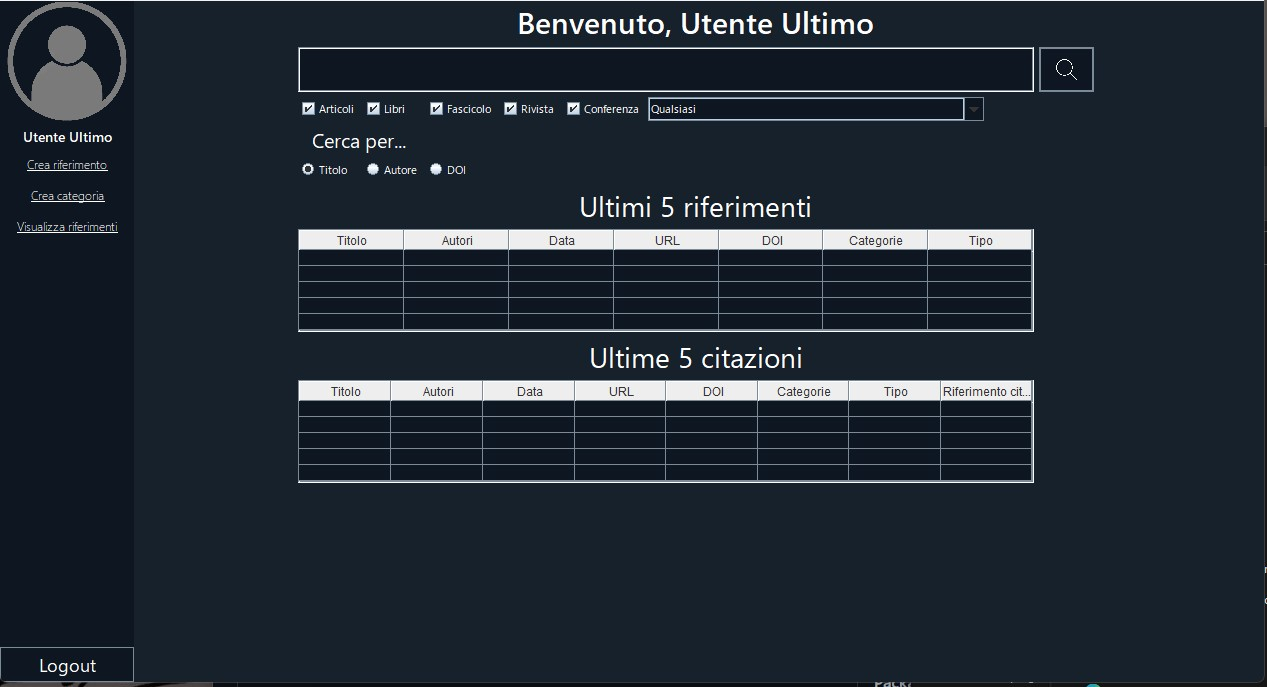
\includegraphics[width=.80\textwidth]{Immagini/VecchioProgetto/homepage.jpg} 

    \caption{Home Page dell'applicativo originale}
\end{figure}

La HomePage del vecchio applicativo ci è sembrato piuttosto ambiguo su alcuni aspetti: che cosa si intende per \textit{Ultimi 5 riferimenti}? Gli ultimi 5 riferimenti creati dall'utente insertiti, gli ultimi 5 riferimenti visualizzati dall'utente, oppure ancora gli ultimi 5 riferimenti inseriti da altri utenti? Discorso analogo per quanto riguarda le citazioni. Abbiamo quindi interpretato che questi fossero delle cronologie delle citazioni e riferimenti inserite dall'utente stesso. Inoltre, si cercherà di migliorare l'affordance generale della schermata, facendo capire a intuito dove inserire il testo per cercare e come cercare.
\\~\\
\begin{figure}[H]
    \centering
            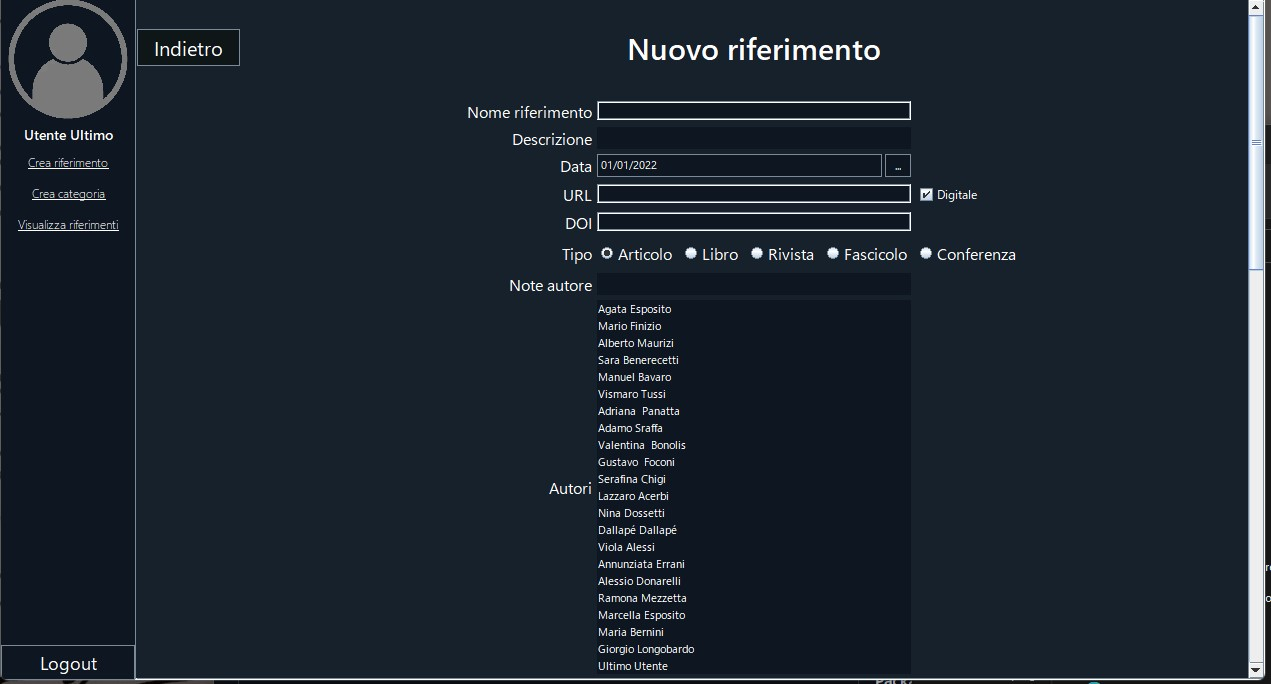
\includegraphics[width=.80\textwidth]{Immagini/VecchioProgetto/crea riferimento.jpg}  

    \caption{Schermata creazione di un nuovo riferimento}
\end{figure}

La schermata originale della creazione di un nuovo riferimento ci è risultata piuttosto confusonaria e alcune sezioni troppo grandi (come la lista degli autori) o troppo piccole (come quella della descrizione). Il nuovo applicativo cercherà di raggruppare tutte queste informazioni in spazi più piccoli e più intuibili, mostrando solamente le informazioni necessarie per l'inserimento.
\begin{figure}[H]
    \centering
            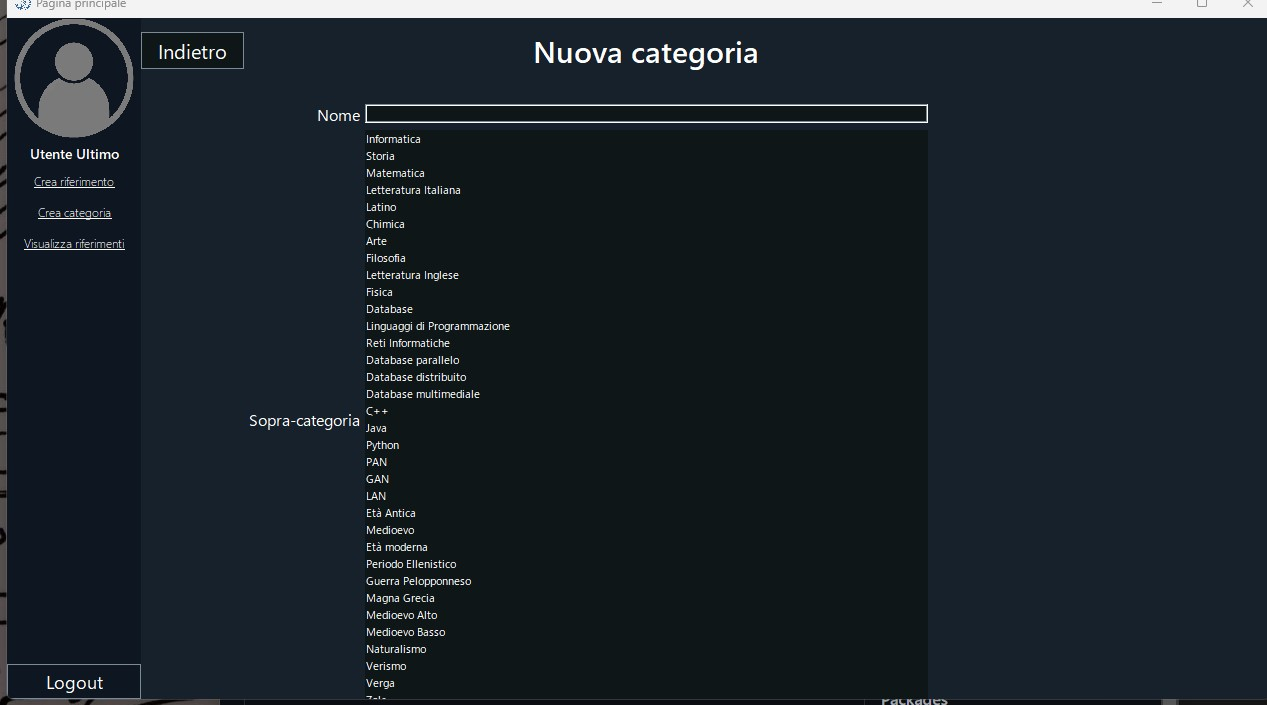
\includegraphics[width=.80\textwidth]{Immagini/VecchioProgetto/crea categoria.jpg}  

    \caption{Schermata creazione di una nuova categoria}
\end{figure}

Discorso analogo vale per la creazione di una categoria, ci è sembrato eccessivo mostrate tutte le sopra-categorie possibili. Essendo molte risulta poi difficoltoso per un utente ricercare quella desiderata.
\begin{figure}[H]
    \centering
            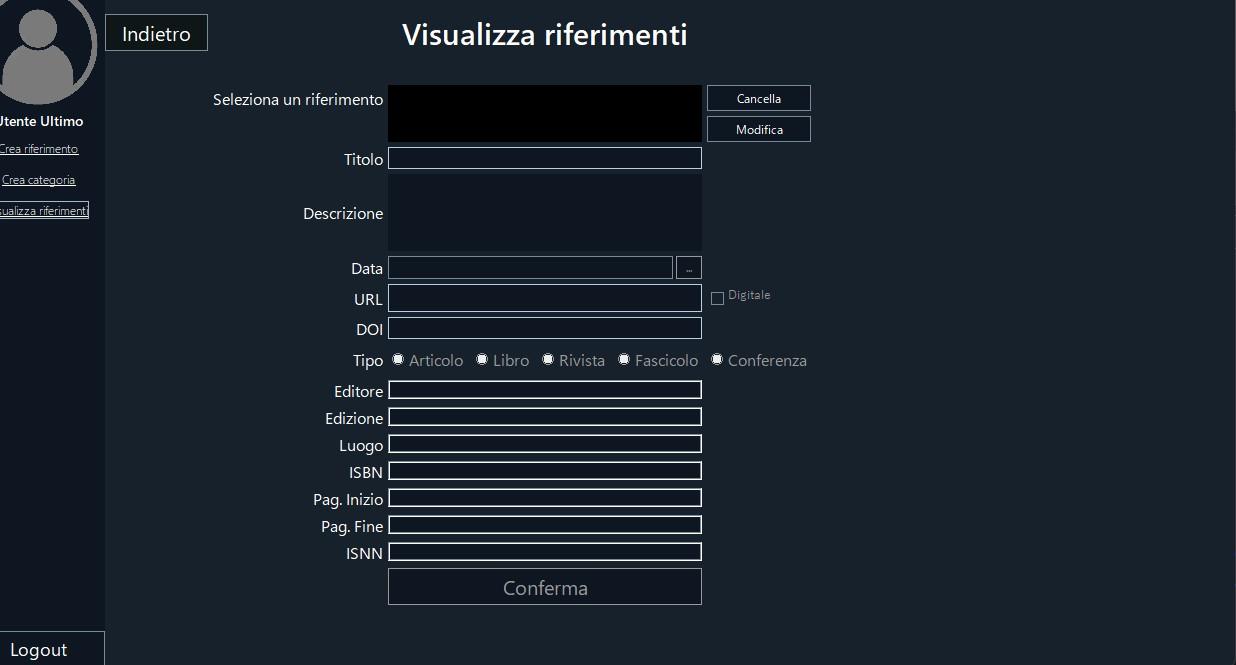
\includegraphics[width=.80\textwidth]{Immagini/VecchioProgetto/visualizza riferimenti.jpg} 

    \caption{Schermata per visualizzare i propri riferimenti}
\end{figure}

La schermata di visualizzazione dei riferimenti è ambigua nel suo nome: non solo è possibile visualizzare tutti i propri riferimenti creati, ma anche modificarli ed eliminarli. Verrà quindi descritto il suo scopo. \\
\raggedright{\subsection{Interfaccia Grafica di Alexandria}}
Di seguito vengono riportati alcuni mock-up delle nuove schermate realizzate per Alexandria.\\
Esse sono state realizzate cercando di rispettare i principi di usabilità e di sfruttare al massimo le icone che esprimono già azioni o immagini universalmente condivise. Per esempio, abbiamo utilizzato l'icona di un omino per esprimere che quel determinato oggetto è un autore e non un riferimento. Abbiamo quindi introdotto una barra di navigazione che godesse di queste proprietà, mediante la quale si possono effettuare inoltre le operazioni più comuni, ponendo al centro la creazione di un riferimento, dato che il centro cattura immediatamente l'occhio. Invece la schermata iniziale sarà principalmente quello per la ricerca, perché è un'altra azione di maggiore utilizzo per la \textit{Alexandria}. Le azioni restanti saranno disponibili o navigando attravero la bottom-bar.
\newpage
 \begin{figure}
\centering
\begin{minipage}{.5\textwidth}
  \centering
  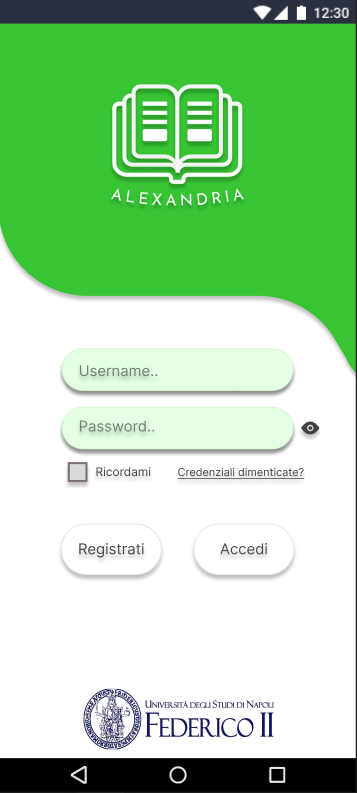
\includegraphics[width=.60\textwidth]{Immagini/Alexandria/Screen/login.PNG} 
\end{minipage}%
\begin{minipage}{.5\textwidth}
\centering
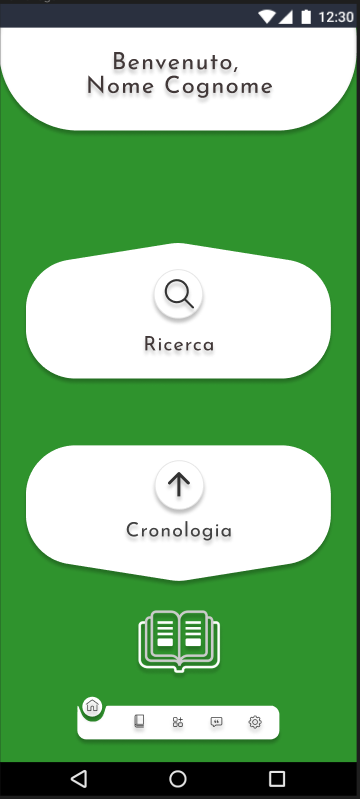
\includegraphics[width=.60\textwidth]{Immagini/Alexandria/Screen/homepage.PNG} 

\end{minipage}
\end{figure}

Queste sono la schermata di accesso e la schermata di homepage. Se si volesse consultare la prototipizzazione completa basta consulatare \href{https://www.figma.com/file/O9LZ0W5HYZAW2BCnP167fL/Alexandria?node-id=0%3A1&t=rqKqdyohunSYcSgf-1}{questo link cliccabile}, dove è annesso il flow dell'applicazione e tutti i frame completi, ognuno realizzato con Figma.


\raggedright{\section{Valutazione dell'usabilità}}
Come già ribadito in precedenza, la nuova interfaccia grafica di Alexandria è stata pensata cercando di rispettare tutti i principi di buona usabilità. Uno dei cambiamenti principali è stato il tema principale dell'applicazione. Attraverso la \href{https://www.my-personaltrainer.it/salute-benessere/la-ruota-delle-emozioni-di-plutchik-cos-e-a-cosa-serve-e-quali-sono-i-suoi-benefici.html}{ruota di Plutchik} abbiamo deciso di assegnare alla nostra nuova applicazione un nuovo colore: il verde chiaro e le sue variazioni. \\~\\
\begin{figure}[H]
    \centering
            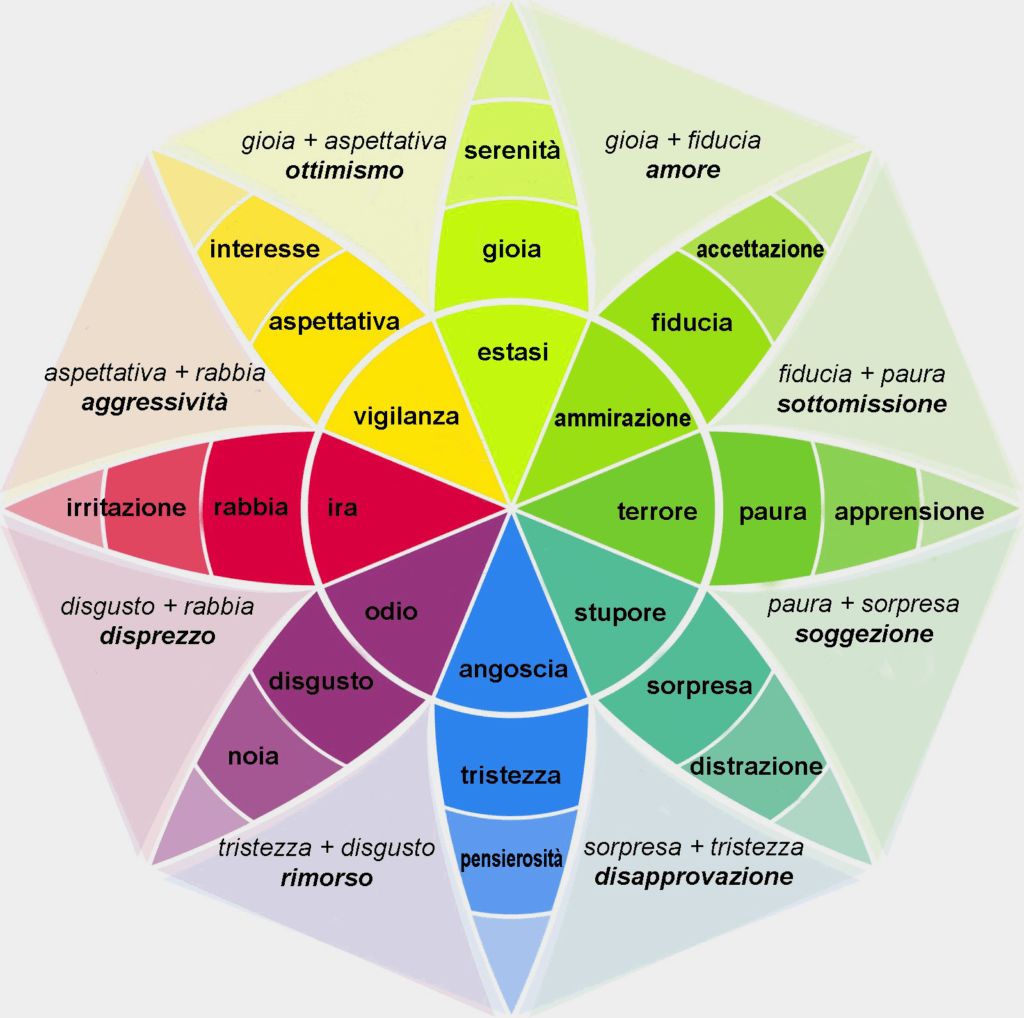
\includegraphics[width=.40\textwidth]{Immagini/Ruota di Plutchik.png} 
    \caption{Ruota di Plutchik}
\end{figure}

Essendo un'applicazione che deve gestire i propri riferimenti, è importante che tale applicazione esprima \textit{Fiducia} nei confronti dell'utente, e consultando la ruota delle emozioni il verde ci è sembrato il colore più adatto alla scelta del tema principale dell'applicazione. \\
Abbiamo inoltre deciso che a schermo non verranno mostrate più informazioni del necessario se non richiesto. Le informaizoni presenti sull'interfaccia grafica sono minimali e riassuntive, per non caricare troppo la memoria a breve termine dell'utente. Inoltre, le icone sono state pensate per rispettare l'uso comune di esse e abbiamo tentato di rendere ogni icona autoesplicativa. Considerato che l'applicativo deve girare su dispositivi mobili, l'interfaccia è stata pensata per apparire su schermi più piccoli, e che quindi l'utente ha una percezione minore rispetto a un monitor: per ovviare a questo problema abbiamo tentato di rendere i pulsanti che creino contrasto con lo sfondo, abbiamo ridotto la quantità di testo per non occupare troppo spazio su schermo, abbiamo preferito uno stile che non sia troppo sfarzoso e ingombrante. Infine, in caso di più pulsanti, essi sono posti distanziati (nei limiti, ovviamente, dei vincoli dell'usabilità e visivi) per evitare che si prema accidentalmente un bottone anziché di un altro, penalizzando l'esperienza dell'utente.
\newpage
\raggedright{\section{Classi, oggetti e relazioni d'analisi}}
Alla luce delle nuove funzionalità da inserire, vengono apportate queste nuove modifiche al Database: 
\begin{figure}[H]
    \centering
            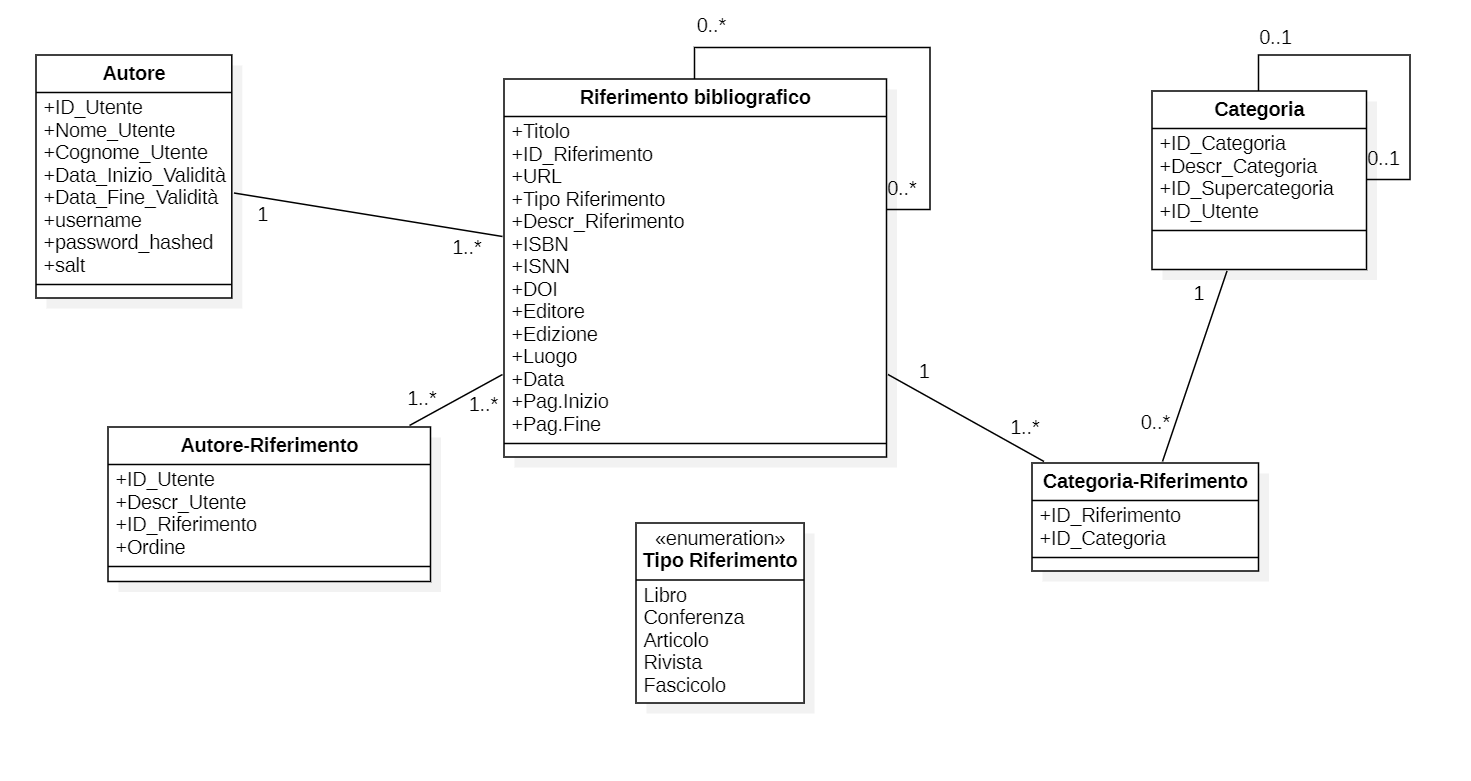
\includegraphics[width=.90\textwidth]{Immagini/Alexandria/UML DB.PNG} 
    \caption{Diagramma delle classi}
\end{figure}

        
La tabella utente ha nuovi attributi: \textit{password hashed}, che contiene la password hashata, \textit{salt}, che servirà per comporre l'hash nel Database e \textit{username}, che serve agli utenti per effettuare il login. Inoltre vengono rimossi gli attributi di \textit{Data Inizio Validità} e \textit{Data Fine Validità} poiché non venivano utilizzati all'interno dell'applicativo e non viene richiesto il suo scopo. Inoltre, alla tabella di associazione \textit{Autore-Riferimento} vengono rimossi gli attributi \textit{Ordine} e \textit{Descrizione Utente}, il primo perché ininfluente ai fini dell'implementazione del Database, il secondo perché ridondante. Per il resto, l'intero sistema ci è sembrato pressoché pertinente allo sviluppo della nuova app reingegnerizzata.

\raggedright{\section{Diagrammi di Sequenza}}
Di seguito vengono riportati i Sequence Diagram di design di due funzionalità: la ricerca di un autore e la creazione di un riferimento. 

\raggedright{\subsection{Diagramma di Sequenza: Ricerca di un Autore}}

Il sequence Diagram qui presente rappresenta l'istante in cui un utente preme su \textit{Ricerca} una volta inseriti tutti i parametri preferiti, supponendo non abbia riscontrato problemi prima di premere invio. 

\raggedright{\subsection{Diagramma di Sequenza: Creazione Riferimento}}

        \begin{center}
            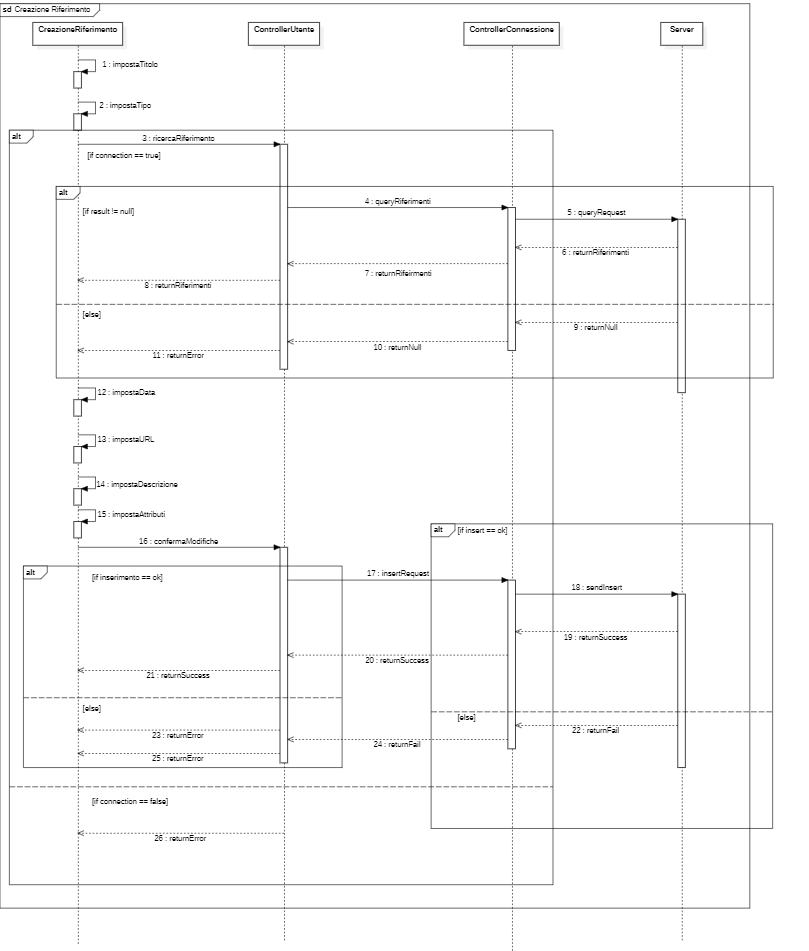
\includegraphics[width=.95\textwidth]{Immagini/Alexandria/sequenceDiagramDesign2.PNG} 
        \end{center}

Il sequence diagram di design qui presente rappresenta l'istante in cui un utente naviga nella finestra dedicata alla creazione di un nuovo riferimento. In particolare, sono stati inseriti tutti i casi di errore e successo.

\raggedright{\section{Prototipazione funzionale}}

\raggedright{\subsection{Statechart: Ricerca Riferimenti}}

        \begin{center}
            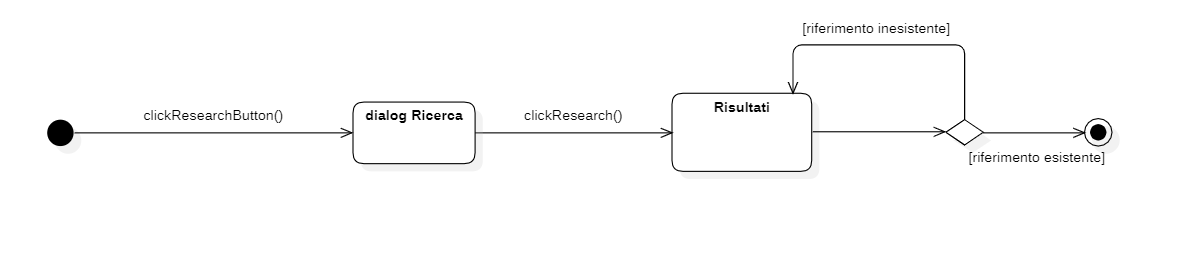
\includegraphics[width=.95\textwidth]{Immagini/Alexandria/Statechart Ricerca.PNG} 
        \end{center}

\raggedright{\subsection{Statechart: Creazione Riferimento}}

        \begin{center}
            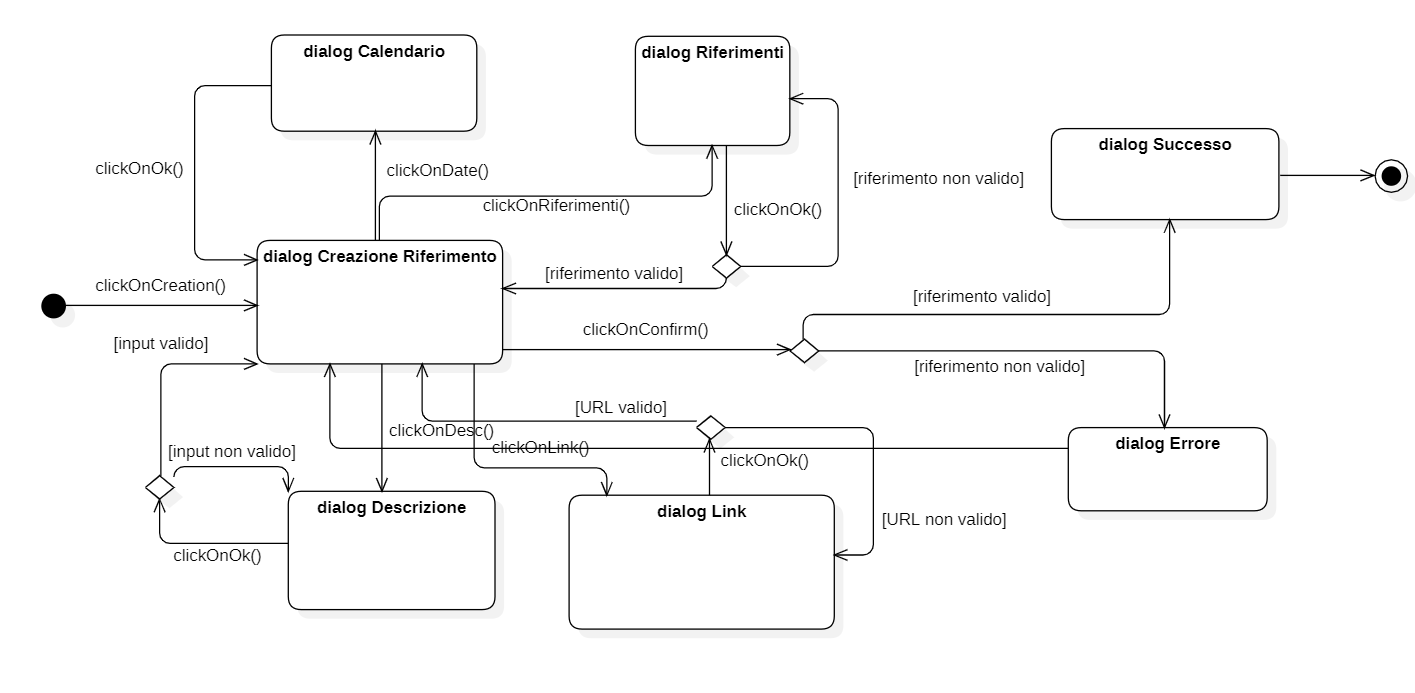
\includegraphics[width=.95\textwidth]{Immagini/Alexandria/Statechart Creazione Riferimento.PNG} 
        \end{center}

\raggedright{\subsection{Statechart: Modifica dei propri Riferimenti}}

        \begin{center}
            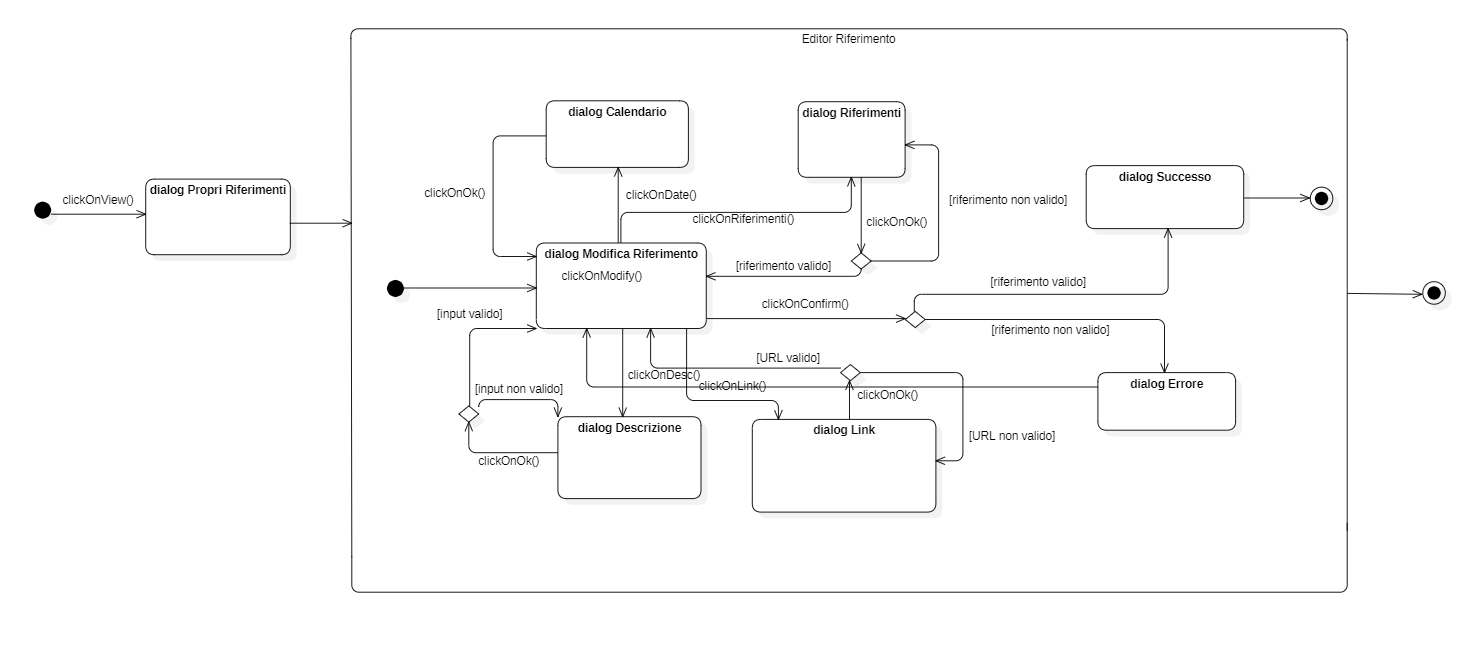
\includegraphics[width=.95\textwidth]{Immagini/Alexandria/Statechart Modifica Riferimento.PNG} 
        \end{center}

\raggedright{\subsection{Statechart: Creazione Categoria}}

        \begin{center}
            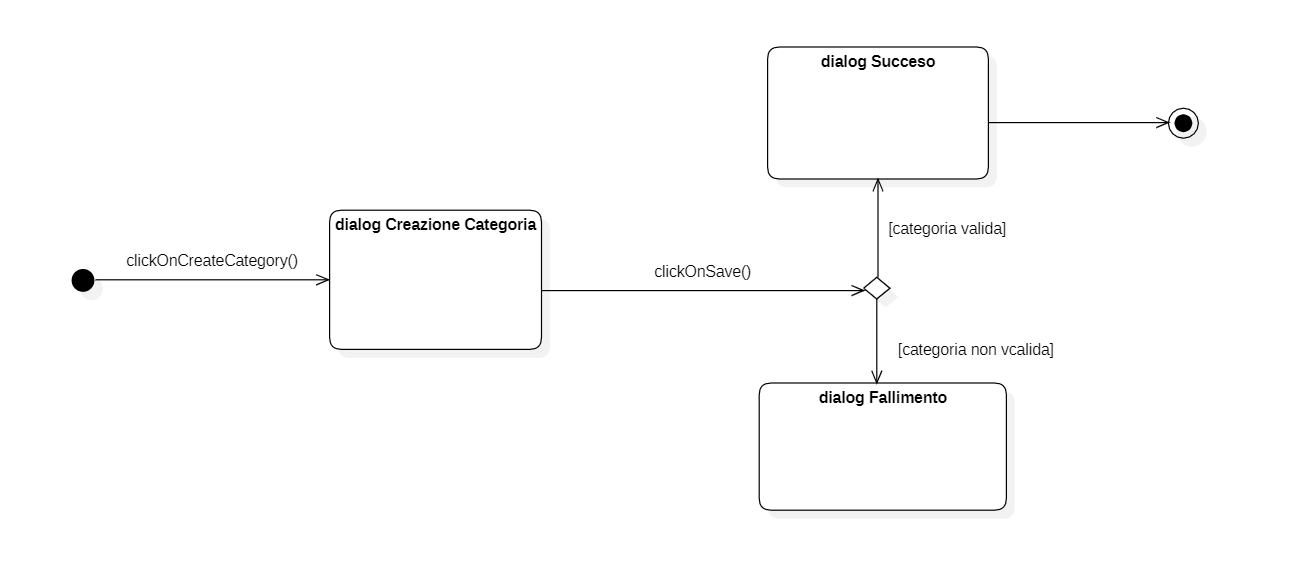
\includegraphics[width=.95\textwidth]{Immagini/Alexandria/Statechart Creazione Categoria.PNG} 
        \end{center}









